\chapter{Reference system transformations}
% File created 19-11-2016 
\label{app:appendixAA-referenceSystemTransformations}
When considering the position, velocity and acceleration of a space vehicle, different reference frames are usually used. Why there are different frames, which frames are required, what they are used for and how to transfer from one frame to the other will be discussed in \Cref{sec:reqrefsys,sec:transfram}. In case of, for instance, a car travelling on the road, a certain coordinate system has to be used to measure the velocity in a certain direction. For the car it can be said that a Cartesian system is used with x in the direction of motion, z pointing towards the ground and y then pointing to the right if looking in the direction of motion (using the so-called \ac{RHR} to complete the frame). The speed is then measured and expressed in the x-direction. This works well when a vehicle is travelling in a straight line or on a flat plane, but in orbital mechanics the motion usually has to be described just above or in an orbit around a (spherical) body. Therefore it is important to know which coordinate system is used and how to change between these coordinate systems should the other system become more convenient to use at a certain point. In \Cref{sec:transsys} the difference between these coordinate systems and how to transfer from one to the other is explained. 


\section{Required reference systems}
\label{sec:reqrefsys}
In the example of the car, the \acf{RF} is fixed to the Earth. However, when considering two cars driving on the same road, one might like to investigate the difference in velocity between both vehicles. In that case an \ac{RF} is chosen that is fixed to one of the two cars. This makes it easier to determine the relative velocity of one car with respect to the other. The same can be done for \ac{s/c} (think of formation flying). There are therefore a number of different \ac{RF}s that can be used. In this section the required \ac{RF}s and their application will be presented.



\subsection{\acl{MCI} \ac{RF} (I-frame)}
\label{subsec:ECI}
The \acf{MCI} reference frame is an \ac{RF} that is, as the name implies, fixed to the centre of mass of Mars \citep{mooij2013fd}. It is a frame in which Mars still rotates with respect to that frame, or in other words it is an inertial frame with respect to Mars. The x-axis is defined through a certain point which can be set by the user. This means that the user can determine his or her own inertial frame. A frame that is often used (and which is based on J2000\footnote{J2000 is an Earth referenced inertial frame that was set through the rotational axis of Earth (z-axis) and through the vernal equinox (x-axis). The reference was set on the Julian date of 2451545.0 or 01-01-2000 at 12:00 \ac{GMT}.}) is the MARSIAU frame \cite{bachman2014naif,diaz2008generic}. This is a Mars inertial frame that is translated from the Earth J2000 frame. For the translation of J2000 a point through the mean equator of Mars is specified where the equator ascends through the mean equator of Earth. The x-axis is defined through this point. The z-axis is then defined through the rotational axis of Mars and the y-axis completes the frame through the \ac{RHR}. The translation is described in \cite{bachman2014naif,diaz2008generic} using the J2000 numbers from \cite{archinal2011report}. The generic inertial frame is shown in \Cref{fig:eci_mooij2013fd}. The centre of the frame is represented by the letter 'A'. The MARSIAU frame is required if certain data from outside sources will have to be incorporated into the simulation, however for the actual simulation and optimisation it will be easier and much more straightforward to define a custom Mars inertial reference frame. 



\begin{figure}[!ht]
\centering
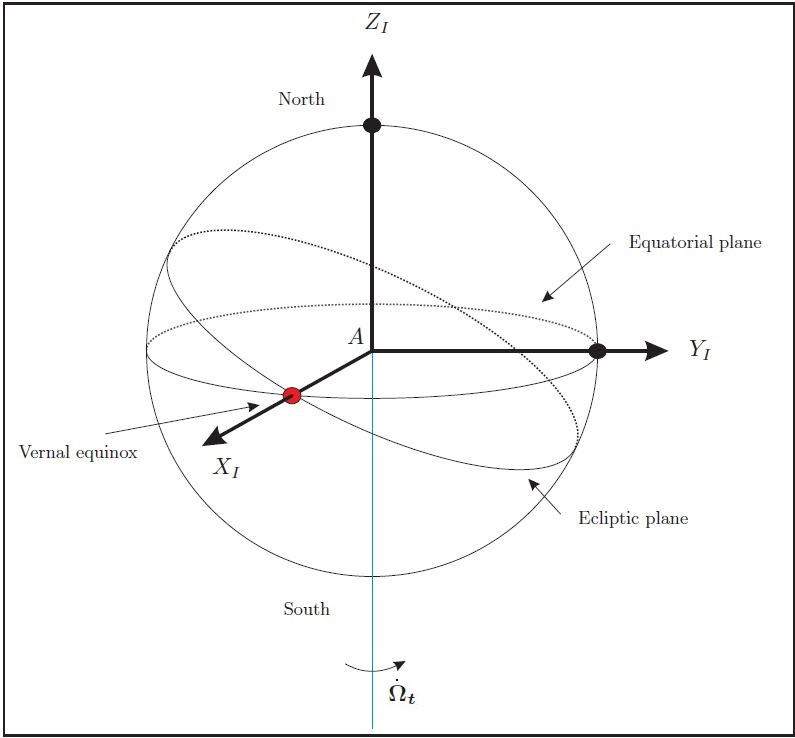
\includegraphics[width=0.5\textwidth]{figures/reference_frames/eci_mooij2013fd.jpg}
\caption{Graphical definition of the Mars-centred inertial reference frame \cite{mooij2013fd}.}
\label{fig:eci_mooij2013fd}
\end{figure}

%\nomenclature{$\Omega_{t}$}{Rotational velocity of Mars\nomunit{rad/s or deg/s}}
%\nomenclature{x$_{I}$}{x-axis of the Mars-centred inertial frame\nomunit{-}}
%\nomenclature{y$_{I}$}{y-axis of the Mars-centred inertial frame\nomunit{-}}
%\nomenclature{z$_{I}$}{z-axis of the Mars-centred inertial frame\nomunit{-}}

This reference system is very useful if the motion of the \ac{s/c} with respect to the ground-track is not important. 




\subsection{\acl{MCMF} \ac{RF} (R-frame)}
\label{subsec:ECEF}
The \acf{MCMF} frame is the same as the \ac{MCI} frame except for one distinct difference. The x-axis of the \ac{MCMF} frame (x$_{R}$) is defined through the 0.5 km wide Airy-0 crater \cite{morton2003mapping} which has a latitude of 5.07829$^{\circ}$S \cite{duxbury2014location}. The associated meridian is called the prime meridian. On 1 January 2000 at 12:00 the prime meridian of Mars was 176.630$^{\circ}$ east of the x-axis in the MARSIAU frame (which is important when transforming from the MARSIAU frame to the current \ac{MCMF} frame)\cite{diaz2008generic,archinal2011report}. Because the Airy-0 crater is fixed to the surface of Mars and rotates around the Martian rotational axis (in both \ac{MCI} and \ac{MCMF} the z-axis), the \ac{MCMF} is also a rotational frame. This frame rotates with Mars and can therefore be very useful for ground observation purposes. In the case of the \ac{MAV} it is important to take the rotational velocity of Mars into account, since Mars will be rotating underneath the \ac{MAV} causing rotational effects. A graphical representation of the \ac{MCMF} frame is provided in \Cref{fig:ecef_mooij2013fd}. An angle $\Omega_{P}$ is defined as the relative angle between the prime meridian and the x-axis of the \ac{MCI} frame at the time that the inertial frame was defined.

%\footnote{ESA website: \url{http://www.esa.int/Our_Activities/Space_Science/Mars_Express/Where_is_zero_degrees_longitude_on_Mars} [Accessed 8 December 2015}]

% The value of this angle thus depends on the definition of the inertial frame.

% When using this reference frame, however, it can also be chosen to not take into account the rotational velocity of Mars. For example, in order for a rover to drive from point A to point B it is not important that this motion is performed on a rotating body.
 
%esa2015where % reference for the 0 longitude on Mars
%duxbury2014location % reference for the latitude of Airy-0
%diaz2008generic % reference for the mentioning of J2000 for Mars in SPICE and also confirms definition of chosen vernal equinox maybe
%archinal2011report % reference for the position of the prime meridian at J2000 with respect to the vernal equinox of J2000 of Mars if they indeed defined it the way I think they did...

\begin{figure}[!ht]
\centering
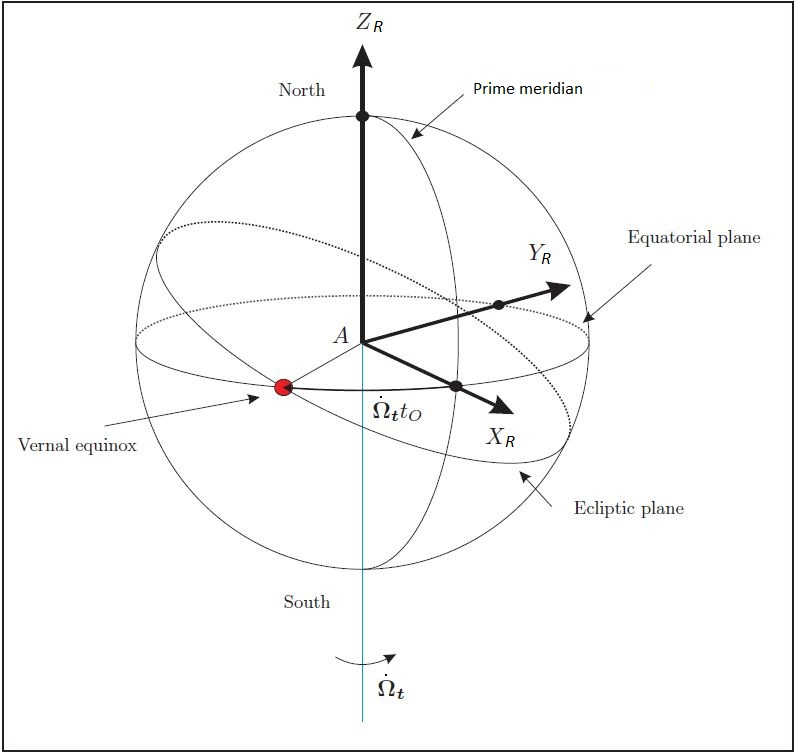
\includegraphics[width=0.4\textwidth]{figures/reference_frames/ecef_mooij2013fd.jpg}
\caption{Graphical definition of the Mars-centred Mars-fixed reference frame \cite{mooij2013fd}. Source: NASA}
\label{fig:ecef_mooij2013fd}
\end{figure}

%\nomenclature{x$_{R}$}{x-axis of the Mars-centred Mars-fixed frame\nomunit{-}}
%\nomenclature{y$_{R}$}{y-axis of the Mars-centred Mars-fixed frame\nomunit{-}}
%\nomenclature{z$_{R}$}{z-axis of the Mars-centred Mars-fixed frame\nomunit{-}}



\subsection{Vertical \ac{RF} (V-frame)}
\label{subsec:VCNE}
This next \ac{RF} can be used to describe the motion of an \ac{s/c} in orbit around a planet. The centre of the vertical frame is defined in the centre of gravity of the \ac{s/c} \cite{mooij2013fd} but is not rotationally fixed to it. This means that the frame can rotate with respect to the \ac{s/c} itself. This is because the x-axis is set to point to the north pole of Mars. The z-axis is perpendicular to Mars' surface (or points to the centre of Mars assuming Mars is a sphere) and the y-axis then points due east. The x-y plane is tangent to Mars' geoid. \Cref{fig:vcne_mooij2013fd} shows the vertical frame denoted by the letter 'V' at an arbitrary position around Mars compared to the \ac{MCI} frame. The centre of the frame is defined by the letter 'G'. The vertical frame relates to the Mars rotational frame through the latitude and longitude. 
%(also see \Cref{fig:spherical_mooij1994motion_force_model_fanning1996model}). 

\begin{figure}[!ht]
\centering
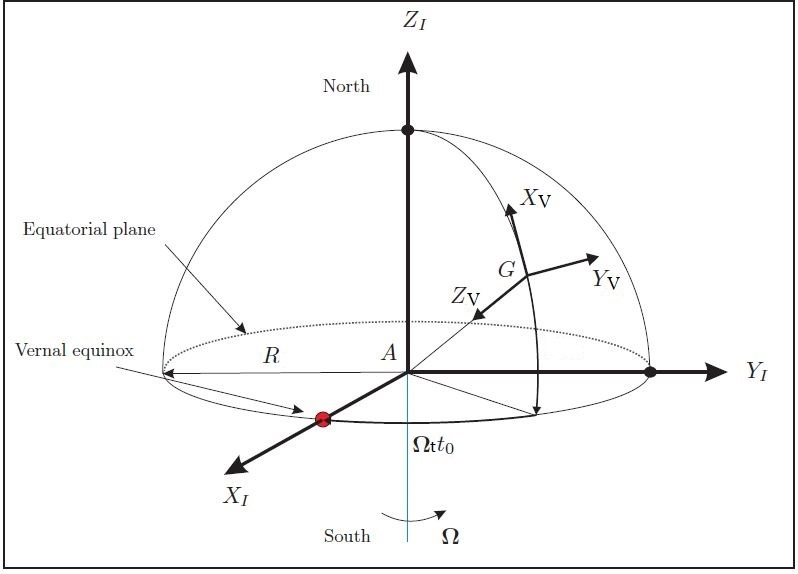
\includegraphics[width=0.5\textwidth]{figures/reference_frames/vcne_mooij2013fd.jpg}
\caption{Graphical definition of the Vertical reference frame compared to the Mars-centred inertial frame \cite{mooij2013fd}.}
\label{fig:vcne_mooij2013fd}
\end{figure} 

%\nomenclature{x$_{V}$}{x-axis of the Vehicle-carried normal Mars frame\nomunit{-}}
%\nomenclature{y$_{V}$}{y-axis of the Vehicle-carried normal Mars frame\nomunit{-}}
%\nomenclature{z$_{V}$}{z-axis of the Vehicle-carried normal Mars frame\nomunit{-}}

%By comparing \Cref{fig:vcne_mooij2013fd} and \Cref{fig:sc_acc_wakker2010} it can be seen that if a spherical Mars is assumed, the accelerations $f_{N}$, $f_{S}$ and $f_{W}$ are oriented in the y$_{V}$, $-$z$_{V}$ and x$_{V}$ direction of the vertical \ac{RF}.

\subsection{\acl{BF} \ac{RF} (B-frame)}
\label{subsec:BF}
The body-fixed \acsu{BF} frame is fixed to the \ac{s/c} body and therefore rotates with the \ac{s/c} as well. The origin of the \ac{BF} \ac{RF} can be defined in the centre of symmetry (or the middle of the \ac{s/c}). The axis orientation can be chosen to be in any direction. In this case the x-axis is defined through the vehicle-centre line and goes through the "nose" of the \ac{s/c}, the z-axis is defined towards the orbiting body (when assuming an orbiting vehicle) and the y-axis completes the frame through the \ac{RHR}. An example of a body frame that can be applied to the \ac{MAV} is provided in \Cref{fig:baseline_liquid_trinidad2012_bframe}. 

%An example of a body frame used for the Apollo Command and Service module is provided in \Cref{fig:csmaxes_woods2009}\footnote{Source: NASA}. In this case the z-axis was however defined by the main hatch of the vehicle.

 

%\begin{figure}[!ht]
%\centering
%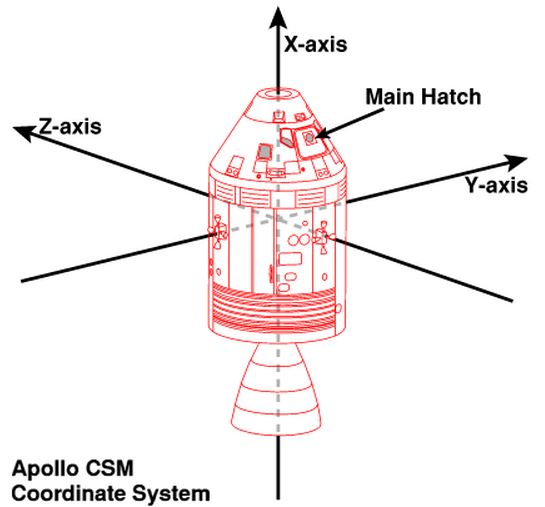
\includegraphics[width=0.3\textwidth]{figures/reference_frames/csmaxes_woods2009.jpg}
%\caption{Graphical example of a Body-fixed reference frame used on the Apollo Command and Service module.}
%\label{fig:csmaxes_woods2009}
%\end{figure}

\begin{figure}[!ht]
\centering
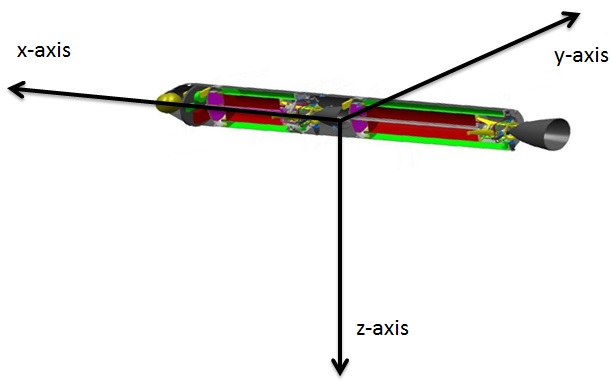
\includegraphics[width=0.6\textwidth]{figures/reference_frames/baseline_liquid_trinidad2012_bframe.jpg}
\caption{Graphical example of a Body-fixed reference frame for the \ac{MAV} \cite{trinidad2012}.}
\label{fig:baseline_liquid_trinidad2012_bframe}
\end{figure}


The axes of the body frame are denoted by a 'B' in this report. In the thesis problem the body frame relates directly to the vertical frame through the flight-path angle $\gamma$ and the heading (or azimuth) angle $\chi$, because the x-axis of the body frame coincides with the velocity vector of the \ac{s/c}. 
%(also see \Cref{fig:spherical_mooij1994motion_force_model_fanning1996model}).



\subsection{Propulsion \ac{RF} (P-frame)}
\label{subsec:propframe}
The propulsion or thrust frame is a body frame where the x-axis is defined by the thrust vector. The y-axis is defined in the same plane as the x and y-axes of the B-frame. Then the z-axis completes the frame through the \ac{RHR} as depicted in \Cref{fig:propframe_mooij1994motion}.

\begin{figure}[!ht]
\centering
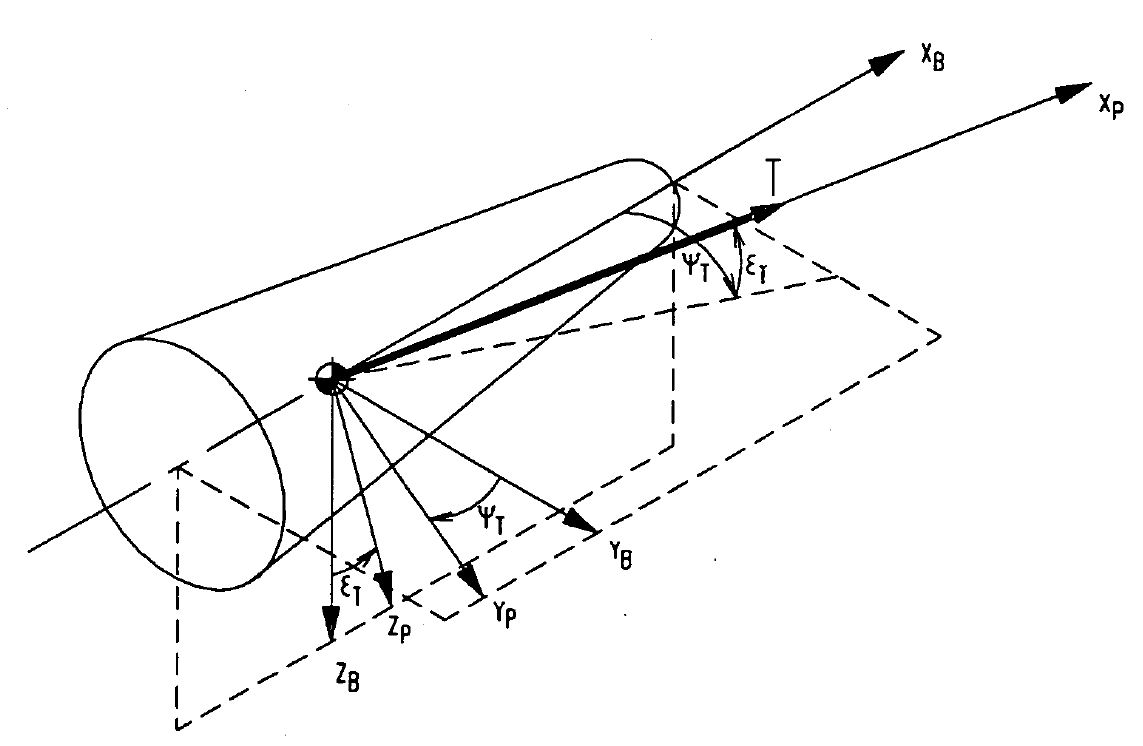
\includegraphics[width=0.6\textwidth]{figures/reference_frames/propframe_mooij1994motion.jpg}
\caption{Propulsion frame relative to the body frame \cite{mooij1994motion}.}
\label{fig:propframe_mooij1994motion}
\end{figure}

The B-frame and P-frame are related through the thrust elevation gimbal angle $\epsilon_{T}$ and the thrust azimuth gimbal angle $\psi_{T}$. 

\section{Transformation between reference frames}
\label{sec:transfram}
Because different problems and situations are easier to understand and to formulate in different \ac{RF}s, it is important to understand how to transform from one \ac{RF} to the other. In this case only transformations for a set point in time, called static transformations, are required for the described thesis problem. The necessary transformations for this thesis problem are described in this section.\\
For a transformation between two \ac{RF}s, a correlation has to exist. This correlation (orientation) can be described using a set of angles, called the Euler angles, between the different \ac{RF}s \cite{mooij2013stat}. In a 3-dimensional space, there are three axes. So to get from one \ac{RF} to the other, a maximum of 3 rotations (translations/transformations) have to take place; one over each axis. However, often fewer rotations are necessary because some of the axes are already properly aligned. Sometimes two reference frames are not directly related through known angles, which means that other (intermediate) \ac{RF}s will have to be used. In this case more than 3 rotations are possible, but again a maximum of three rotations are needed to go from one \ac{RF} to an intermediate \ac{RF} given the known angles. Since a 3-dimensional space is described, 3-dimensional coordinates have to be translated to the next reference frame. For this, Cartesian coordinates are used. A rotation around the x-axis can be described by the change in the y- and z-coordinates over an angle $\phi$ in the yz-plane as visualized in \Cref{fig:xtrans_mooij2013stat}. The rotation around the x-axis follows the \ac{RHR} of rotation, which states that if the thumb of your right hand is pointed in the axis direction, then the rest of your fingers show the direction of positive orientation. Therefore the described rotation is positive. Should the rotation have been in the other direction (clockwise around the x-axis as seen in \Cref{fig:xtrans_mooij2013stat}), the angle would have been negative. This is very important in transformations, and its usefulness becomes more obvious when more transformations are performed after each other. But first a system of equations is required to transform from the 'i' frame to the 'j' frame. 



\nomenclature[G7]{$\phi$}{General rotation angle\nomunit{rad}}


\begin{figure}[!ht]
\centering
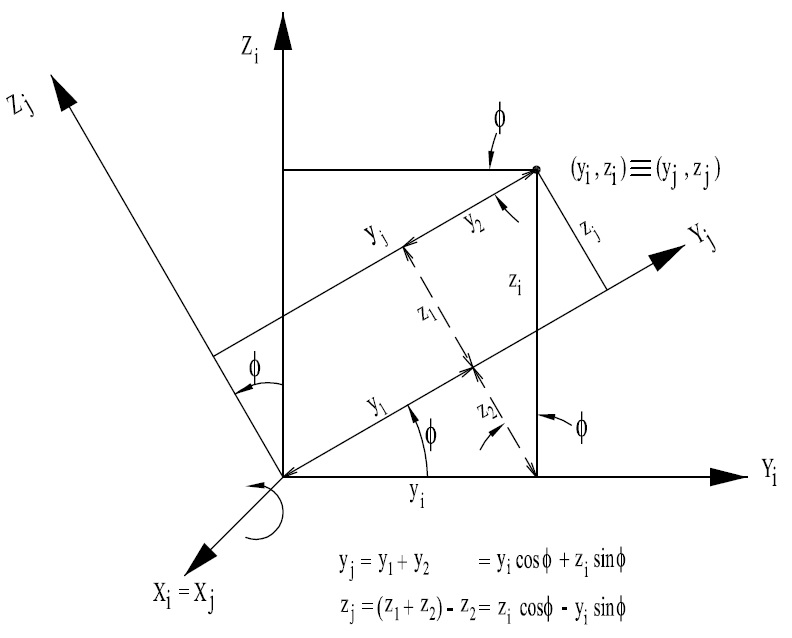
\includegraphics[width=0.6\textwidth]{figures/reference_frames/xtrans_mooij2013stat.jpg}
\caption{General rotation around the x-axis \cite{mooij2013stat}.}
\label{fig:xtrans_mooij2013stat}
\end{figure}

From \Cref{fig:xtrans_mooij2013stat}  a relation can be described between the coordinates in the 'i' frame and the 'j' frame in matrix form. This relation (convention as by \cite{mooij2013stat}) is shown by \Cref{eq:xaxistransmatr}. Here, $\mathbf{r}$ is the position vector and $\mathbb{T}_{\mathbf{x}}(\phi)$ represents the x-axis transformation matrix and is the standard matrix to be used if a transformation around an x-axis is performed. The only parameter that changes is the angle.

\nomenclature[Ra0]{$\mathbf{r}$}{Position vector \nomunit{m}}
\nomenclature[S1]{$\mathbb{T}$}{General transformation matrix\nomunit{-}}
%\nomenclature{$\mathbb{T}_{\mathbf{x}}$}{x-axis transformation matrix\nomunit{-}}
%\nomenclature{$$}{\nomunit{}}

\begin{equation} \label{eq:xaxistransmatr}
\begin{pmatrix}
x\\
y\\
z\\
\end{pmatrix}_{j}=
\begin{bmatrix}
1 & 0 & 0 \\
0 & \cos\phi & \sin\phi \\
0 & -\sin\phi & \cos\phi \\
\end{bmatrix}
\begin{pmatrix}
x\\
y\\
z\\
\end{pmatrix}_{i}\Rightarrow
\mathbf{r}_{j}=\mathbb{T}_{\mathbf{x}}(\phi)\mathbf{r}_{i}
\end{equation}


This rotation described by \Cref{fig:xtrans_mooij2013stat} and \Cref{eq:xaxistransmatr} can also be described for rotations around the y-axis and the z-axis. The complete set of axis transformation matrices is then presented in \Cref{eq:alltransmatr}.

\begin{equation} \label{eq:alltransmatr}
\mathbb{T}_{\mathbf{x}}(\phi)=\begin{bmatrix}
1 & 0 & 0 \\
0 & \cos\phi & \sin\phi \\
0 & -\sin\phi & \cos\phi \\
\end{bmatrix}, 
\mathbb{T}_{\mathbf{y}}(\phi)=\begin{bmatrix}
\cos\phi & 0 & -\sin\phi \\
0 & 1 & 0\\
\sin\phi & 0 & \cos\phi \\
\end{bmatrix}, 
\mathbb{T}_{\mathbf{z}}(\phi)=\begin{bmatrix}
\cos\phi & \sin\phi & 0\\
- \sin\phi & \cos\phi & 0\\
0 & 0 & 1\\
\end{bmatrix}
\end{equation}

From now on, the cosine notation will be shortened to 'c' and the sine notation will be shortened to 's' to make the transformation matrices more comprehensive. Also, because the matrices are orthogonal, the inverse of the matrix is simply the transpose of the matrix. The inverse of a rotation matrix is the rotation in the other direction.\\
The order, or sequence, in which these transformations are performed is very important. This is because the sequence results in a matrix multiplication equation, and from linear algebra it is known that $\mathbf{A}\cdot\mathbf{B}\neq\mathbf{B}\cdot\mathbf{A}$. Therefore, if the sequence of transformations is not correct, the resulting \ac{RF} will not be the desired \ac{RF}.  Also, as mentioned before, it is not always possible or easy to transform from one \ac{RF} directly into the other. So usually one of the afore mentioned \ac{RF} is used as an intermediate \ac{RF}. It is therefore possible to transform from the P-frame all the way to the I-frame using all the other mentioned \ac{RF}s with a maximum of three rotations between each frame. For convenience it has been chosen to adopt the convention mentioned in \cite{mooij2013fd} and \cite{mooij2013stat} to describe the transformations. Therefore the I-frame, R-frame, V-frame, B-frame and P-frame will be known as $F_{I}$, $F_{R}$, $F_{V}$, $F_{B}$ and $F_{P}$ respectively when used to indicate the \ac{RF}s in equations. And because these equations involve matrix multiplications, they have to be executed from right to left. Therefore it can be said that the transformation matrix to go from $F_{B} \rightarrow F_{R}$ is $\mathbb{T}_{\mathbf{RB}}=\mathbb{T}_{\mathbf{RV}}\mathbb{T}_{\mathbf{VB}}$. This is one of the transformations required for the \ac{MAV} trajectory. The other two transformations are more straightforward: $F_{P} \rightarrow F_{B}$ is $\mathbb{T}_{\mathbf{BP}}$ and $F_{R} \rightarrow F_{I}$ is $\mathbb{T}_{\mathbf{IR}}$. For the $\mathbb{T}_{\mathbf{IR}}$ matrix , a transition is performed from $F_{R} \rightarrow F_{I}$. This is done over the angle $\dot{\Omega}_{t}t_{O}$ as defined in \Cref{fig:ecef_mooij2013fd}. $\dot{\Omega}_{t}$ is the rotational velocity of Mars and $t_{O}$ is the time from the set inertial frame. This is also where $\Omega_{P0}$ is required (not depicted) since this angle describes the position of the prime meridian at the time that the inertial frame was set. Because the angle is defined east of the x$_{I}$-axis, it has to be subtracted from $\dot{\Omega}_{t}t_{O}$ since $\Omega_{P0}$ is defined positive in the same direction as $\dot{\Omega}_{t}t_{O}$ which is defined to be positive going from x$_{I}$ to x$_{R}$. The rotation around the z-axis is positive in the same direction according to the \ac{RHR} for rotation. In this case the rotation is performed in the negative direction around the z-axis with an angle $-\dot{\Omega}_{M}t_{O}+\Omega_{P}$. The complete \ac{RF} transformation with the written out matrix for this rotation is given by \Cref{eq:IRtrans}. Please note that the signs of the angles changed in the matrix due to the sine and cosine functions.

\begin{equation} \label{eq:IRtrans}
\mathbb{T}_{\mathbf{IR}}=\Bigg|_{\mathbf{I}}\mathbb{T}_{\mathbf{z}}\left(-\dot{\Omega}_{M}t_{O}+\Omega_{P}\right)\Bigg|_{\mathbf{R}}=
\begin{bmatrix}
c\left(\dot{\Omega}_{M}t_{O}-\Omega_{P}\right) & -s\left(\dot{\Omega}_{M}t_{O}-\Omega_{P}\right) & 0\\
s\left(\dot{\Omega}_{M}t_{O}-\Omega_{P}\right) & c\left(\dot{\Omega}_{M}t_{O}-\Omega_{P}\right) & 0\\
0& 0& 1\\
\end{bmatrix}
\end{equation}

Here the vertical lines with the letter designations depict when a certain reference frame is reached. The transformations for $\mathbb{T}_{\mathbf{RB}}$ and $\mathbb{T}_{\mathbf{BP}}$ can now be written in a similar manner and are described in \Cref{eq:RBtrans,eq:BPtrans} respectively.

\begin{multline} \label{eq:RBtrans}
\mathbb{T}_{\mathbf{RB}}=\Bigg|_{\mathbf{R}}\mathbb{T}_{\mathbf{z}}\left(-\tau\right)\mathbb{T}_{\mathbf{y}}\left(\dfrac{\pi}{2}+\delta\right)\Bigg|_{\mathbf{V}}\mathbb{T}_{\mathbf{z}}\left(-\chi\right)\mathbb{T}_{\mathbf{y}}\left(-\gamma\right)\Bigg|_{\mathbf{B}}\\
=
\begin{bmatrix}
c\tau\left(-s\delta c\chi c\gamma +c\delta s\gamma \right)-s\tau s\chi c\gamma  & c\tau s\delta s\chi -s\tau c\chi & c\tau\left(-s\delta c\chi s\gamma -c\delta c\gamma \right)-s\tau s\chi s\gamma \\
s\tau\left(-s\delta c\chi c\gamma +c\delta s\gamma \right)+c\tau s\chi c\gamma  & s\tau s\delta s\chi +c\tau c\chi & s\tau\left(-s\delta c\chi s\gamma -c\delta c\gamma \right)+c\tau s\chi s\gamma \\
c\delta c\chi c\gamma -c\delta s\gamma  & -c\delta s\chi &  c\delta c\chi s\gamma -s\delta c\gamma \\
\end{bmatrix}
\end{multline}

%\begin{bmatrix}
%c\left(-\tau\right) & s\left(-\tau\right) & 0\\
%-s\left(-\tau\right) & c\left(-\tau\right) & 0\\
%0 & 0 & 1\\
%\end{bmatrix}
%\begin{bmatrix}
%c\left(\dfrac{\pi}{2}+\delta\right) & 0 & -s\left(\dfrac{\pi}{2}+\delta\right)\\
%0 & 1 & 0\\
%s\left(\dfrac{\pi}{2}+\delta\right) & 0 & c\left(\dfrac{\pi}{2}+\delta\right)\\
%\end{bmatrix}
%\begin{bmatrix}
%c\left(-\chi\right) & s\left(-\chi\right) & 0\\
%-s\left(-\chi\right) & c\left(-\chi\right) & 0\\
%0 & 0 & 1\\
%\end{bmatrix}
%\begin{bmatrix}
%c\left(-\gamma\right) & 0 & -s\left(-\gamma\right)\\
%0 & 1 & 0\\
%s\left(-\gamma\right) & 0 & c\left(-\gamma\right)\\
%\end{bmatrix}=\\
%\begin{bmatrix}
%c\left(\tau\right) & -s\left(\tau\right) & 0\\
%s\left(\tau\right) & c\left(\tau\right) & 0\\
%0 & 0 & 1\\
%\end{bmatrix}
%\begin{bmatrix}
%-s\delta  & 0 & -c\left(\delta\right)\\
%0 & 1 & 0\\
%c\left(\delta\right) & 0 & -s\left(\delta\right)\\
%\end{bmatrix}
%\begin{bmatrix}
%c\chi  & -s\left(\chi\right) & 0\\
%s\left(\chi\right) & c\left(\chi\right) & 0\\
%0 & 0 & 1\\
%\end{bmatrix}
%\begin{bmatrix}
%c\gamma  & 0 & s\left(\gamma\right)\\
%0 & 1 & 0\\
%-s\left(\gamma\right) & 0 & c\left(\gamma\right)\\
%\end{bmatrix}=\\
%\begin{bmatrix}
%c\left(\tau\right) & -s\left(\tau\right) & 0\\
%s\left(\tau\right) & c\left(\tau\right) & 0\\
%0 & 0 & 1\\
%\end{bmatrix}
%\begin{bmatrix}
%-s\left(\delta\right) & 0 & -c\left(\delta\right)\\
%0 & 1 & 0\\
%c\left(\delta\right) & 0 & -s\left(\delta\right)\\
%\end{bmatrix}
%\begin{bmatrix}
%c\left(\chi\right)c\left(\gamma\right) & -s\left(\chi\right) & c\left(\chi\right)s\left(\gamma\right)\\
%s\left(\chi\right)c\left(\gamma\right) & c\left(\chi\right) & s\left(\chi\right)s\left(\gamma\right)\\
%-s\left(\gamma\right) & 0 & c\left(\gamma\right)
%\end{bmatrix}=\\
%\begin{bmatrix}
%c\left(\tau\right) & -s\left(\tau\right) & 0\\
%s\left(\tau\right) & c\left(\tau\right) & 0\\
%0 & 0 & 1\\
%\end{bmatrix}
%\begin{bmatrix}
%-s\left(\delta\right)c\left(\chi\right)c\left(\gamma\right)+c\left(\delta\right)s\left(\gamma\right) & s\left(\delta\right)s\left(\chi\right) & -s\left(\delta\right)c\left(\chi\right)s\left(\gamma\right)-c\left(\delta\right)c\left(\gamma\right)\\
%s\left(\chi\right)c\left(\gamma\right) & c\left(\chi\right) & s\left(\chi\right)s\left(\gamma\right)\\
%c\left(\delta\right)c\left(\chi\right)c\left(\gamma\right)-c\left(\delta\right)s\left(\gamma\right) & -c\left(\delta\right)s\left(\chi\right) & c\left(\delta\right)c\left(\chi\right)s\left(\gamma\right)-s\left(\delta\right)c\left(\gamma\right)\\ 
%\end{bmatrix}=\\
%\left[
%\begin{matrix}
%c\tau\left(-s\delta c\chi c\gamma +c\delta s\gamma \right)-s\tau s\chi c\gamma  & c\tau s\delta s\chi -s\tau c\chi \\
%s\tau\left(-s\delta c\chi c\gamma +c\delta s\gamma \right)+c\tau s\chi c\gamma  & s\tau s\delta s\chi +c\tau c\chi \\
%c\delta c\chi c\gamma -c\delta s\gamma  & -c\delta s\chi \\
%\end{matrix}\right.
%\\
%\left.
%\begin{matrix}
%c\tau\left(-s\delta c\chi s\gamma -c\delta c\gamma \right)-s\tau s\chi s\gamma \\
%s\tau\left(-s\delta c\chi s\gamma -c\delta c\gamma \right)+c\tau s\chi s\gamma \\
% c\delta c\chi s\gamma -s\delta c\gamma \\
%\end{matrix}\right]


\begin{equation} \label{eq:BPtrans}
\mathbb{T}_{\mathbf{BP}}=\Bigg|_{\mathbf{B}}\mathbb{T}_{\mathbf{z}}\left(-\psi_{T}\right)\mathbb{T}_{\mathbf{y}}\left(-\epsilon_{T}\right)\Bigg|_{\mathbf{P}}=
\begin{bmatrix}
c\psi_{T}c\epsilon_{T} & -s\psi_{T} & c\psi_{T}s\epsilon_{T}\\
s\psi_{T}c\epsilon_{T} & c\psi_{T} & s\psi_{T}s\epsilon_{T}\\
-s\epsilon_{T} & 0 & c\epsilon_{T}
\end{bmatrix}
\end{equation}

%\begin{bmatrix}
%c\left(-\psi_{T}\right) & s\left(-\psi_{T}\right) & 0\\
%-s\left(-\psi_{T}\right) & c\left(-\psi_{T}\right) & 0\\
%0 & 0 & 1\\
%\end{bmatrix}
%\begin{bmatrix}
%c\left(-\epsilon_{T}\right) & 0 & --\left(-\epsilon_{T}\right)\\
%0 & 1 & 0\\
%s\left(-\epsilon_{T}\right) & 0 & c\left(-\epsilon_{T}\right)\\
%\end{bmatrix}=\\
%\begin{bmatrix}
%c\left(\psi_{T}\right) & -s\left(\psi_{T}\right) & 0\\
%s\left(\psi_{T}\right) & c\left(\psi_{T}\right) & 0\\
%0 & 0 & 1\\
%\end{bmatrix}
%\begin{bmatrix}
%c\left(\epsilon_{T}\right) & 0 & s\left(\epsilon_{T}\right)\\
%0 & 1 & 0\\
%-s\left(\epsilon_{T}\right) & 0 & c\left(\epsilon_{T}\right)\\
%\end{bmatrix}=



Occasionally transformation matrices can become rather complex and it is easy to make mistakes. Fortunately the motion of the orbiter is already known in Kepler (or Modified Equinoctial) elements. This means that for the gravitational accelerations caused by the Sun described in \Cref{eq:third_b_per}, which are in the \ac{MCI} \ac{RF}, they can be directly transformed to the body-fixed $f_{S}$, $f_{N}$ and $f_{W}$ \ac{RF}. From now on this \ac{RF} is referred to as the Gaussian frame or $F_{G}$, which can be similar to the $F_{V}$ frame but does not have to be. The transformation from $F_{I} \rightarrow F_{G}$ follows from \Cref{fig:sc_acc_wakker2010_repeat} and is provided by the transformation convention and matrices described by \Cref{eq:ItoG}. In this case an intermediate reference frame is required which will be called $F_{I"}$, because two z-axis rotations are needed, but they are not in the same plane. It can also be seen that the position of the Prime meridian  on the 1$^{st}$ of January 2000 at 12:00 is not important in this direct transformation and will only have to be taken into account in the transformation from $F_{R} \leftrightarrow F_{I}$ for the \ac{MAV}.



\begin{figure}[!ht]
\centering
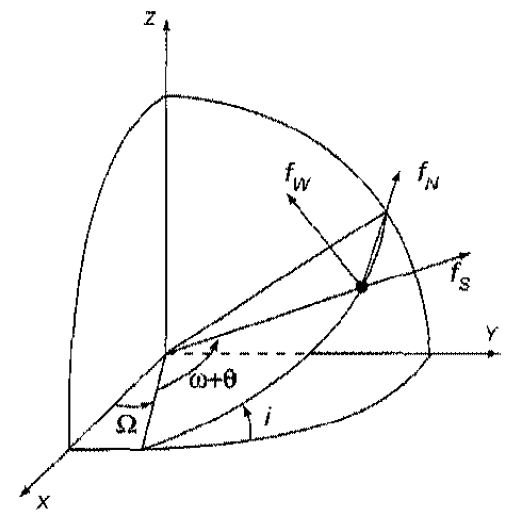
\includegraphics[width=0.3\textwidth]{figures/transfer_orbits/sc_acc_wakker2010.jpg}
\caption{Relation between the \ac{MCI} and the Gaussian body frame \cite{wakker2010}.}
\label{fig:sc_acc_wakker2010_repeat}
\end{figure}

%\begin{equation} \label{eq:ItoGseq}
%\mathbb{T}_{\mathbf{GI}}=\mathbb{T}_{\mathbf{GI"}}\mathbb{T}_{\mathbf{I"I}}=
%\Bigg|_{\mathbf{G}}\mathbb{T}_{\mathbf{z}}(\omega+\theta)\Bigg|_{\mathbf{I"}}\mathbb{T}_{\mathbf{x}}(i)\mathbb{T}_{\mathbf{z}}(\Omega)\Bigg|_{\mathbf{I}}
%\end{equation} 




\begin{multline} \label{eq:ItoG}
\mathbb{T}_{\mathbf{GI}}=\mathbb{T}_{\mathbf{GI"}}\mathbb{T}_{\mathbf{I"I}}=
\Bigg|_{\mathbf{G}}\mathbb{T}_{\mathbf{z}}(\omega+\theta)\Bigg|_{\mathbf{I"}}\mathbb{T}_{\mathbf{x}}(i)\mathbb{T}_{\mathbf{z}}(\Omega)\Bigg|_{\mathbf{I}}\\
=
\begin{bmatrix}
c(\omega+\theta)c\Omega -s(\omega+\theta)ci s\Omega  & c(\omega+\theta)s\Omega +s(\omega+\theta)ci c\Omega  & s(\omega+\theta)si \\
-s(\omega+\theta)c\Omega -c(\omega+\theta)ci s\Omega  & c(\omega+\theta)ci c\Omega -s(\omega+\theta)s\Omega  & c(\omega+\theta)si \\
si s\Omega  & -si c\Omega  & ci \\
\end{bmatrix}
\end{multline}

%\begin{bmatrix}
%c(\omega+\theta) & s(\omega+\theta) & 0\\
%-s(\omega+\theta) & c(\omega+\theta) & 0 \\
%0 & 0 & 1\\
%\end{bmatrix}
%\begin{bmatrix}
%1 & 0 & 0\\
%0& c(i)& s(i)\\
%0 & -s(i) & c(i)\\
%\end{bmatrix}
%\begin{bmatrix}
%c(\Omega) & s(\Omega) & 0\\
%-s(\Omega) & c(\Omega) & 0\\
% 0 & 0 & 1\\
%\end{bmatrix}\\
%=
%\begin{bmatrix}
%c(\omega+\theta) & s(\omega+\theta) & 0\\
%-s(\omega+\theta) & c(\omega+\theta) & 0 \\
%0 & 0 & 1\\
%\end{bmatrix}
%\begin{bmatrix}
%c(\Omega) & s(\Omega) & 0\\
%-c(i)s(\Omega) & c(i)c(\Omega) & s(i)\\
%s(i)s(\Omega) & -s(i)c(\Omega) & c(i)\\
%\end{bmatrix}\\



\section{Transformation between different coordinate systems}
\label{sec:transsys}
In the previous sections the different \ac{RF} and transformations were expressed using x, y and z-axes. These x, y and z-coordinates belong to the Cartesian coordinate system. However, during an integration, simulation or analysis it might be more useful and meaningful to express position (and velocity) in a different coordinate system. Two other systems are the spherical and Keplerian coordinate systems. How to transform back and forth from the Cartesian system to these other two systems will be explained in \Cref{subsec:sphercart,subsec:keplcart} respectively and are based on \cite{noomen2013basic}. The transformation from the spherical coordinate system to Kepler elements is described in \Cref{subsec:spherkepl}. Kepler elements are very useful for orbit computations, unfortunately singularities can occur if this coordinate system is used for certain situations. Therefore \Cref{subsec:nosingkep} will discuss a non-singular form of the Kepler elements. 

\subsection{Spherical and Cartesian}
\label{subsec:sphercart}
Spherical coordinates can be useful to determine the location of a satellite above Mars assuming that Mars is a perfect sphere. In this thesis problem, however, spherical coordinates are used during the \ac{MAV} ascent simulation. The coordinate relation between spherical and Cartesian coordinates is shown in \Cref{fig:sphertocart_noomen2013basic}. Based on this diagram, the relations to go from the spherical system to the Cartesian system are derived and are provided in \Cref{eq:sphertocartp}. Please note that $\lambda\neq\tau$ except for a transformation to (or from) the R-frame.

\begin{figure}[!ht]
\centering
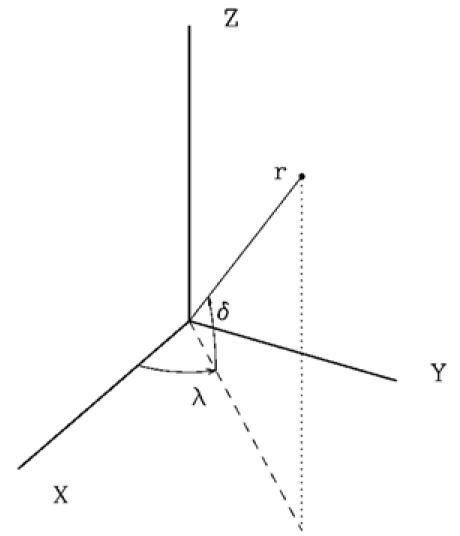
\includegraphics[width=0.3\textwidth]{figures/reference_frames/sphertocart_noomen2013basic.jpg}
\caption{Relation between spherical position coordinates and Cartesian position coordinates \cite{noomen2013basic}.}
\label{fig:sphertocart_noomen2013basic}
\end{figure}

%\nomenclature{$r$}{Radius\nomunit{m}}

\begin{equation} \label{eq:sphertocartp}
\begin{split}
& x=r\cos\delta \cos(\lambda \\
& y=r\cos\delta \sin(\lambda \\
& z=r\sin\delta 
\end{split}
\end{equation}

The velocities can be obtained by taking the time derivatives of these functions, resulting in the velocity expressions in x-, y- and z-direction given by \Cref{eq:sphertocartv}. Differentiating those expressions again will result in the accelerations.

\begin{equation} \label{eq:sphertocartv}
\begin{split}
& \dot{x}=\dot{r}\cos\delta \cos(\lambda -r\dot{\delta}\sin\delta \cos(\lambda -r\dot{\lambda}\cos\delta \sin(\lambda \\
& \dot{y}=\dot{r}\cos\delta \sin(\lambda -r\dot{\delta}\sin\delta \sin(\lambda +r\dot{\lambda}\cos\delta \cos(\lambda \\
& \dot{z}=\dot{r}\sin\delta +r\dot{\delta}\cos\delta 
\end{split}
\end{equation}

The transformation from Cartesian coordinates to spherical coordinates can again be derived from \Cref{fig:sphertocart_noomen2013basic}, resulting in the expressions presented in \Cref{eq:carttospherp}.

\begin{equation} \label{eq:carttospherp}
\begin{split}
& r=\sqrt{x^{2}+y^{2}+z^{2}}\\
& \delta=\arcsin(\dfrac{z}{r})\\
& \lambda=\arctan(\dfrac{y}{x})
\end{split}
\end{equation}

However, the expression for $\lambda$ only results in a value between $-\pi/2$ and $\pi/2$. Also, if x = 0, a singularity occurs. To solve this issue, the so-called 'atan2' function can be used. This function incorporates both sin and cosine values to provide a value for $\lambda$ between 0 and 2$\pi$ \cite{noomen2013basic}. $\lambda$ can then be expressed by \Cref{eq:simpatan2} where atan2 is defined by \Cref{fig:atan2_guilhaire2013}\footnote{Online blog: \url{http://guihaire.com/code/?p=1168} [Accessed 13 November 2015]}.

\begin{equation} \label{eq:simpatan2}
\lambda=\text{atan}2(y,x)
\end{equation}

%The actual definitions behind atan2 are given in \Cref{fig:atan2_guilhaire2013}.

\begin{figure}[!ht]
\centering
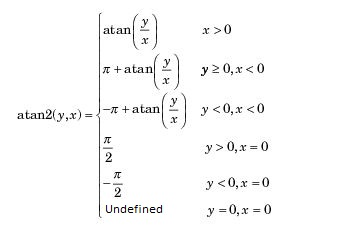
\includegraphics[width=0.5\textwidth]{figures/reference_frames/atan2_guilhaire2013.jpg}
\caption{atan2 function evaluation conditions.}
\label{fig:atan2_guilhaire2013}
\end{figure}

The time derivatives of these functions can be taken to find the velocity expressions. The resulting velocity expressions are shown in \Cref{eq:carttospherv}. The left expressions in this equation define the velocity characteristics as often expressed in the spherical coordinate system required for transformations.

%\begin{equation} \label{eq:carttospherv}
%\begin{split}
%& \dot{r}=\dfrac{x\dot{x}+y\dot{y}+z\dot{z}}{\sqrt{x^{2}+y^{2}+z^{2}}}\\
%& \dot{\delta}=\dfrac{x\dot{y}-y\dot{x}}{x^{2}+y^{2}}\\
%& \dot{\lambda}=\dfrac{r\dot{z}-z\dot{r}}{r^{2}\sqrt{1-\left(\dfrac{z}{r}\right)^{2}}}
%\end{split}
%\end{equation}
%
%From these expression, the values for $V$, $\gamma$ and $\chi$ can be computed using the expressions provided in \Cref{eq:restspher}.
%
%\begin{equation} \label{eq:restspher}
%\begin{split}
%V&=\sqrt{\dot{x}^{2}+\dot{y}^{2}+\dot{z}^{2}}\\
%\gamma&=\arcsin\left[\dfrac{\dot{r}}{V}\right]\\
%\chi&=\arccos\left[\dfrac{r \dot{\delta}}{V\cos\left(\gamma\right)}\right]
%\end{split}
%\end{equation}

\begin{align} \label{eq:carttospherv}
\begin{split}
& \dot{r}=\dfrac{x\dot{x}+y\dot{y}+z\dot{z}}{\sqrt{x^{2}+y^{2}+z^{2}}}\\
& \dot{\delta}=\dfrac{x\dot{y}-y\dot{x}}{x^{2}+y^{2}}\\
& \dot{\lambda}=\dfrac{r\dot{z}-z\dot{r}}{r^{2}\sqrt{1-\left(\dfrac{z}{r}\right)^{2}}}
\end{split}
&
\begin{split}
V&=\sqrt{\dot{x}^{2}+\dot{y}^{2}+\dot{z}^{2}}\\
\gamma&=\arcsin\left[\dfrac{\dot{r}}{V}\right]\\
\chi&=\arccos\left[\dfrac{r \dot{\delta}}{V\cos\gamma }\right]
\end{split}
\end{align}


\subsection{Keplerian and Cartesian}
\label{subsec:keplcart}
The relation between the Keplerian and Cartesian systems is slightly more complex. \Cref{fig:kepler_noomen2013basic_akcasu2013_1} shows the Kepler elements: $a$ (semi-major axis), $e$ (eccentricity, not shown but is a ratio that determines the elliptic properties of an orbit), $i$ (inclination), $\omega$ (argument of perigee), $\Omega$ (right ascension of the ascending node) and $\theta$ (true anomaly). Often, however, the mean anomaly $M$ is used instead of the true anomaly. The mean anomaly is defined to be the angle between the semi-major axis and the line between the centre of the orbit and an imaginary point ($S_{M}$) on the auxiliary circle that can be drawn around the orbit. This point is determined by assuming a constant rotational velocity in this circular orbit with the same orbital time as the actual (elliptical) orbit. 


\nomenclature[R8]{$M$}{Mean anomaly\nomunit{rad}}

\begin{figure}[!ht]
\centering
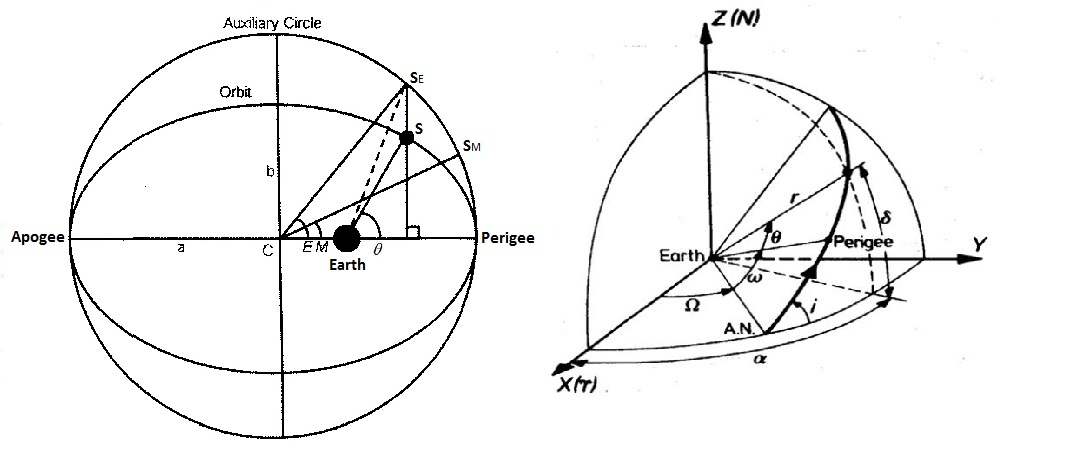
\includegraphics[width=1.0\textwidth]{figures/reference_frames/kepler_noomen2013basic_akcasu2013.jpg}
\caption{Definition of the Kepler elements in 2D (left) and 3D (right) \cite{noomen2013basic,akcasu2013}.}
\label{fig:kepler_noomen2013basic_akcasu2013_1}
\end{figure}

The transformation from Kepler elements to Cartesian coordinates consists of a number of steps starting with the mean anomaly and eccentricity. Both these values have to be used to determine the eccentric anomaly $E$ and in turn the true anomaly $\theta$. The eccentric anomaly is computed by rewriting the first expression of \Cref{eq:mandecomp} into the second expression \cite{noomen2013basic}. 

\nomenclature[R2]{$E$}{Eccentric anomaly\nomunit{rad}}
%\nomenclature{$\theta$}{True anomaly\nomunit{rad}}


\begin{equation}\label{eq:mandecomp}
\begin{split}
 M&=E-e\cdot\sin{E}\\
 E_{i+1}&=E_{i}+\dfrac{M-E_{i}-e\cdot\sin{E_{i}}}{1-e\cdot\cos(E_{i})}
\end{split}
\end{equation}


The determination of $E$ is an iterative process. First a reasonable estimate of $E$ has to be provided (it is best to use the value for $M$ for this) and then a new $E$ can be computed. This has to be done until the desired level of precision is reached. Then the true anomaly can be computed using this $E$ as shown by \Cref{eq:etothetacomp}.

\begin{equation}\label{eq:etothetacomp}
\theta=2\cdot\arctan\left[\tan\left(\dfrac{E}{2}\right)\sqrt{\dfrac{1+e}{1-e}}\right]
\end{equation}

With the true anomaly known, the radial distance from the orbiting body to the centre of Mars $r$ can be determined using \Cref{eq:radiuscomp}

\begin{equation}\label{eq:radiuscomp}
r=\dfrac{a\cdot(1-e^{2})}{1+e\cos\theta }
\end{equation}

The Cartesian coordinates can now be computed using the expression in \Cref{eq:keptocartmat} with the matrix entries provided by \Cref{eq:matrixent}\cite{noomen2013basic}. 

\begin{equation}\label{eq:keptocartmat}
\begin{pmatrix}
x\\
y\\
z\\
\end{pmatrix}=
\begin{bmatrix}
l_{1} & l_{2}\\
m_{1} & m_{2}\\
n_{1} & n_{2}\\
\end{bmatrix}
\begin{pmatrix}
r\cos\theta \\
r\sin\theta \\
\end{pmatrix}
\end{equation}

\begin{equation}\label{eq:matrixent}
\begin{split}
 l_{1}&=\cos\Omega \cos\omega -\sin\Omega \sin\omega \cos i \\
 l_{2}&=-\cos\Omega \sin\omega -\sin\Omega \cos\omega \cos i \\
 m_{1}&=\sin\Omega \cos\omega +\cos\Omega \sin\omega \cos i \\
 m_{2}&=-\sin\Omega \sin\omega +\cos\Omega \cos\omega \cos i \\
 n_{1}&=\sin\omega \sin i \\
 n_{2}&=\cos\Omega \sin i 
\end{split}
\end{equation}

\noindent \Cref{eq:keptocartp} then provides the expressions for x, y and z.

\begin{equation}\label{eq:keptocartp}
\begin{split}
 x&=r\cdot[\cos\Omega \cos(\omega+\theta)-\sin\Omega \sin(\omega+\theta)\cos i ]\\
 y&=r\cdot[\sin\Omega \cos(\omega+\theta)-\cos\Omega \sin(\omega+\theta)\cos i ]\\
 z&=r\sin i \sin(\omega+\theta)
\end{split}
\end{equation}
 
For the velocity values, an extra parameter is required. This parameter is called the specific relative angular momentum $h$. Assuming that the mass of the orbiting body can be neglected with respect to the planet (or other celestial body) it is orbiting, $h$ can be expressed as a function of the standard gravitational parameter of that planet $\mu$, $a$ and $e$ as shown by \Cref{eq:anglmomhktoc}.

\nomenclature[R4]{$h$}{Specific relative angular momentum\nomunit{m$^{2}$/s}}
\nomenclature[G5]{$\mu$}{Standard gravitational parameter\nomunit{m$^{3}$/s$^{2}$}}


\begin{equation}\label{eq:anglmomhktoc}
h=\sqrt{\mu a\cdot(1-e^{2})}
\end{equation}   

Then with $h$ and the expression from \Cref{eq:matrixent}, the velocities can be expressed by \Cref{eq:keptocartv}.

\begin{equation}\label{eq:keptocartv}
\begin{split}
 \dot{x}&=\dfrac{\mu}{h}[-l_{1}\sin\theta +l_{2}\cdot(e+\cos\theta )]\\
 \dot{y}&=\dfrac{\mu}{h}[-m_{1}\sin\theta +m_{2}\cdot(e+\cos\theta )]\\
 \dot{z}&=\dfrac{\mu}{h}[-n_{1}\sin\theta +n_{2}\cdot(e+\cos\theta )]
\end{split}
\end{equation}

%\begin{equation}\label{eq:keptocartv}
%\begin{split}
% \dot{x}&=\dfrac{\mu}{h}[\left(\sin(\Omega)\sin\omega \cos(i)-\cos(\Omega)\cos(\omega)\right)\sin(\theta)-\left(\cos(\Omega)\sin(\omega)+\sin(\Omega)\cos(\omega)\right)(e+\cos(\theta))]\\
% \dot{y}&=\dfrac{\mu}{h}[-\left(\sin(\Omega)\cos(\omega)+\cos(\Omega)\sin(\omega)\cos(i)\right)\sin(\theta)+\left(\cos(\Omega)\cos(\omega)-\sin(\Omega)\sin(\omega)\right)(e+\cos(\theta))]\\
% \dot{z}&=\dfrac{\mu}{h}[-\sin(\omega)\sin(i)\sin(\theta)+\cos(\Omega)\sin(i)(e+\cos(\theta))]
%\end{split}
%\end{equation}


It is also possible to convert from the Cartesian system back to the Kepler system, however, this requires more steps and intermediate expressions. First, it is convenient to express the position and velocity both in one vector each as shown by \Cref{eq:randvvectors}.

\begin{equation}\label{eq:randvvectors}
\begin{split}
\mathbf{r}&=\begin{bmatrix}
x & y & z\\
\end{bmatrix}\\
\mathbf{V}&=\begin{bmatrix}
\dot{x} & \dot{y} & \dot{z}\\
\end{bmatrix}
\end{split}
\end{equation}

The cross product of these two ($\mathbf{r}\times\mathbf{V}$) will result in the specific relative angular momentum vector $\mathbf{h}$ and the scalar values, or lengths, can then be represented by $r=\|\mathbf{r}\|$, $V=\|\mathbf{V}\|$ and $h=\|\mathbf{h}\|$. Also, a vector $\mathbf{N}$ can be defined as shown by \Cref{eq:N}\cite{noomen2013basic}.

\begin{equation}\label{eq:N}
\mathbf{N}=\begin{pmatrix}
0\\
0\\
1\\
\end{pmatrix}
\times
\mathbf{h}
\end{equation}

With these parameters set, the first four Kepler elements ($a$, $e$, $i$ and $\Omega$) can be computed as shown by \Cref{eq:carttokep4}. Here, the value for the eccentricity can be obtained by taking the length of the vector: $e=\|\mathbf{e}\|$. Also, $\mathbf{h}(3)$ is the third value of the specific relative angular momentum vector, so the value in the z-direction. The same principle holds for the values from $\mathbf{N}$.

\begin{equation}\label{eq:carttokep4}
\begin{split}
a&=\left(\dfrac{2}{r}-\dfrac{V^{2}}{\mu}\right)^{-1}\\
\mathbf{e}&=\dfrac{\mathbf{V} \times \mathbf{h}}{\mu}-\dfrac{\mathbf{r}}{r}\\
i&=\arccos\left(\dfrac{\mathbf{h}(3)}{h}\right)\\
\Omega&=\text{atan}2\left(\mathbf{N}(2),\mathbf{N}(1)\right)
\end{split}
\end{equation}

For the computation of the values for $\omega$ and $\theta$, three unit vectors are needed: $\hat{\mathbf{N}}=\dfrac{\mathbf{N}}{\|\mathbf{N}\|}$, $\hat{\mathbf{e}}=\dfrac{\mathbf{e}}{\|\mathbf{e}\|}$ and $\hat{\mathbf{r}}=\dfrac{\mathbf{r}}{\|\mathbf{r}\|}$. This leads to the conditional expressions seen in \Cref{eq:omegathetacond}. 



\begin{equation}\label{eq:omegathetacond}
\begin{split}
\omega&=\begin{cases}
\arccos\left(\hat{\mathbf{e}}\cdot\hat{\mathbf{N}}\right), & \text{if } \left(\hat{\mathbf{N}} \times \mathbf{e}\right) \cdot \mathbf{h}>0\\
-\arccos\left(\hat{\mathbf{e}}\cdot\hat{\mathbf{N}}\right), & \text{otherwise}
\end{cases}\\
\theta&=\begin{cases}
\arccos\left(\hat{\mathbf{r}}\cdot\hat{\mathbf{e}}\right), & \text{if } \left(\mathbf{e} \times \mathbf{r}\right) \cdot \mathbf{h}>0\\
-\arccos\left(\hat{\mathbf{r}}\cdot\hat{\mathbf{e}}\right), & \text{otherwise}
\end{cases}
\end{split}
\end{equation}

The eccentric anomaly can now be computed using $\theta$ and $e$ as shown by \Cref{eq:ecc}, which is the rewritten form of \Cref{eq:etothetacomp}.

\begin{equation}\label{eq:ecc}
E=2\cdot\arctan\left[\tan\left(\dfrac{\theta}{2}\right)\sqrt{\dfrac{1-e}{1+e}}\right]
\end{equation}

And finally, the mean anomaly can be found using \Cref{eq:mandecomp}\cite{noomen2013basic}.



\subsection{Spherical and Keplerian}
\label{subsec:spherkepl}
Often it is required to transform the spherical coordinates into Kepler elements. Wakker \cite{wakker2010astro1} provides this direct transformation through the relations provided in \Cref{eq:sphertokepl}. In this case the expressions are written explicitly for Mars by using $\mu_{M}$.

%At the end of the ascent phase, the spherical coordinates will have to be transformed to the normal Kepler elements to be able to compare the position and velocity of the \ac{MAV} to that of the Mars 2022 orbiter. 

\begin{equation} \label{eq:sphertokepl}
\begin{split}
a&=\dfrac{r}{2-\dfrac{rV^{2}}{\mu_{M}}}\\
e&=\sqrt{1-\dfrac{rV^{2}}{\mu_{M}}\left(2-\dfrac{rV^{2}}{\mu_{M}}\right)\cos^{2}\gamma }\\
i&=\arccos\left(\cos\delta \sin\chi \right)\\
\theta&=2\arctan\left[\sqrt{\dfrac{1+e}{1-e}}\tan\left(\dfrac{E}{2}\right)\right], \qquad \text{where} \qquad E=\arctan\left[\sqrt{\dfrac{a}{\mu_{M}}}\dfrac{rV\sin\gamma }{a-r}\right] \\
\omega&=\dfrac{\sin\delta }{\sin\left(i\right)}-\theta\\
\Omega&=\lambda-\arccos\left[\dfrac{\cos\chi }{\sin\left(i\right)}\right]\\
\end{split}
\end{equation}   

Then the spherical coordinates can be computed by rewriting the expressions provided in \Cref{eq:sphertokepl} to the spherical coordinates. These rewritten expressions are shown in \Cref{eq:kepltospher}. 

\begin{equation} \label{eq:kepltospher}
\begin{split}
r&= a\left(1-e\cos\left(E\right)\right), \qquad \text{where} \qquad E=2\arctan\left[\sqrt{\dfrac{1-e}{1+e}}\tan\left(\dfrac{\theta}{2}\right)\right]\\
V&=\sqrt{\mu_{M}\left(\dfrac{2}{r}-\dfrac{1}{a}\right)}\\
\gamma&=\arcsin\left[e\sin\left(E\right)\dfrac{\sqrt{\mu_{M}a}}{rV}\right]\\
\delta&=\arcsin\left[\sin\left(\omega+\theta\right)\sin\left(i\right)\right]\\
\lambda&=\arcsin\left[\dfrac{\tan\delta }{\tan\left(i\right)}\right]-\Omega\\
\chi&=\arccos\left[\cos\left(\omega+\theta\right)-\dfrac{\sin\left(i\right)}{\cos\delta }\right]\\
\end{split}
\end{equation} 


\subsection{Non-singular Kepler elements}
\label{subsec:nosingkep}
During the calculation of the change in orbital elements, sometimes a number of Kepler elements cannot assume every possible value. Singularities occur when $e=0$, and/or $i=0^{\circ}$ or $180^{\circ}$. One kind of non-singular Kepler elements are the \ac{MEE}s. The transformation from the ordinary Kepler elements to the \ac{MEE}s is shown in \Cref{eq:keplttomee_and_meetokepl}. This equation also includes the expressions to revert back to normal Kepler elements (see left equations). Here  $I$ is the retrograde factor and has a value of +1 for posigrade orbits and -1 for retrograde orbits. This is done to avoid singularities when $i=180^{\circ}$ and thus making the set non-singular. 




%\begin{equation} \label{eq:kepltomee}
%\begin{split}
%p&=a\left(1-e^{2}\right)\\
%f&=e\cos\left(\omega+I\Omega\right)\\
%g&=e\sin\left(\omega+I\Omega\right)\\
%h&=\tan^{I}\left(\dfrac{i}{2}\right)\cos\left(\Omega\right)\\
%k&=\tan^{I}\left(\dfrac{i}{2}\right)\sin\left(\Omega\right)\\
%L&=\omega+\theta+I\Omega\\
%\end{split}
%\end{equation}
%
%These expressions can be reverted back into normal Kepler elements by using the expressions provided in \Cref{eq:meetokepl}. 
%
%\begin{equation}\label{eq:meetokepl}
%\begin{split}
%a&=\dfrac{p}{1-\left(f^{2}+g^{2}\right)}\\
%e&=\sqrt{f^{2}+g^{2}}\\
%i&=2\tan^{-I}\left[\sqrt{h^{2}+k^{2}}\right]\\
%\omega&=L-\theta-I\Omega\\
%\Omega&=atan2\left(k,h\right)\\
%\theta&=L-\arccos\left[\dfrac{f}{e}\right]
%\end{split}
%\end{equation}


\begin{align} \label{eq:keplttomee_and_meetokepl}
\begin{split}
p&=a\left(1-e^{2}\right)\\
f&=e\cos\left(\omega+I\Omega\right)\\
g&=e\sin\left(\omega+I\Omega\right)\\
h&=\tan^{I}\left(\dfrac{i}{2}\right)\cos\left(\Omega\right)\\
k&=\tan^{I}\left(\dfrac{i}{2}\right)\sin\left(\Omega\right)\\
L&=\omega+\theta+I\Omega\\
\end{split}
&
\begin{split}
a&=\dfrac{p}{1-\left(f^{2}+g^{2}\right)}\\
e&=\sqrt{f^{2}+g^{2}}\\
i&=2\tan^{-I}\left[\sqrt{h^{2}+k^{2}}\right]\\
\omega&=L-\theta-I\Omega\\
\Omega&=\text{atan}2\left(k,h\right)\\
\theta&=L-\arccos\left[\dfrac{f}{e}\right]
\end{split}
\end{align}




